\documentclass{IEEEcsmag}
\usepackage[colorlinks,urlcolor=blue,linkcolor=blue,citecolor=blue]{hyperref}
\usepackage{todonotes}

\usepackage{booktabs}
\usepackage{comment}
\usepackage{upmath}
\usepackage{hyperref}
\usepackage[strict]{changepage}
\usepackage[framemethod=TikZ]{mdframed}
% for formal definitions
\usepackage{framed}

\newcommand{\secref}[1]{\nameref{#1}}

\long\def\gnote#1{{[[[[\textbf{\color{red}#1 -Gustavo}]]]]}}

% environment derived from framed.sty: see leftbar environment definition
\definecolor{formalshade}{rgb}{0.95,0.95,1}

\newenvironment{formal}{%
  \def\FrameCommand{%
    \hspace{1pt}%
    {\color{formalshade}\vrule width 2pt}%
    {\color{formalshade}\vrule width 4pt}%
    \colorbox{formalshade}%
  }%
  \MakeFramed{\advance\hsize-\width\FrameRestore}%
  \noindent\hspace{-4.55pt}% disable indenting first paragraph
  \begin{adjustwidth}{}{7pt}%
  \vspace{2pt}\vspace{2pt}%
}
{%
  \vspace{2pt}\end{adjustwidth}\endMakeFramed%
}

\jvol{XX}
\jnum{XX}
\paper{8}
\jmonth{August}
\jname{IT Professional}
\pubyear{2020}
\newtheorem{theorem}{Theorem}
\newtheorem{lemma}{Lemma}

\setcounter{secnumdepth}{0}

\begin{document}

\sptitle{Department: Head}
\editor{Editor: Name, xxxx@email}

\title{Breaking one barrier at a time: how women developers cope in a men-dominated industry}

\newcommand{\orcidauthorEdna}{0000-0002-2159-339X} % Edna
\newcommand{\orcidauthorFabiana}{0000-0002-1724-2044} % Fabiana
\newcommand{\orcidauthorAnderson}{0000-0002-6973-3240} % Anderson
\newcommand{\orcidauthorGustavo}{0000-0001-7598-2799} % Anderson

\author{Edna Dias Canedo \textsuperscript{\orcidauthorEdna{}}}
\affil{Department of Computer Science, University of Bras\'{i}lia (UnB), Bras\'{i}lia--DF, Brazil}

\author{Fabiana Freitas Mendes \textsuperscript{\orcidauthorFabiana{}}}
\affil{Faculty UnB Gama, University of Bras\'{i}lia (UnB), Bras\'{i}lia--DF, Brazil}

\author{Anderson Jefferson Cerqueira \textsuperscript{\orcidauthorAnderson{}}}
\affil{Department of Computer Science, University of Bras\'{i}lia (UnB), Bras\'{i}lia--DF, Brazil}

\author{M\'{a}rcio Vinicius Okimoto}
\affil{Department of Computer Science, University of Bras\'{i}lia (UnB), Bras\'{i}lia--DF, Brazil}

\author{Gustavo Pinto \textsuperscript{\orcidauthorGustavo{}}}
\affil{Federal University of Par\'{a} (UFPA), Par\'{a}--PA, Brazil}

\markboth{Department Head}{Paper title}

\begin{abstract}
Women are underrepresented in software development teams. %\cite{StackOverflow,DBLP:conf/vl/FordHP17,esem2020}
We investigate the women perception in relation to interactions, contributions, gender bias, barriers and challenges that they may face in their work. The findings indicate that most of the interviewed women observe a sexist behavior amongst the software development team members. Moreover, most of the participants stated that few women perform a leadership role in their team. We close by presenting suggestions to more inclusive work environments. 
\end{abstract}

\maketitle

%The presence of women in an organization depends on the characteristics of that organization, such as: size, prestige, relations with public and private organizations, and opportunities for career growth. On the other hand, practitioners' motivation depends on their position in the labor market and in the organization in which they operate. Women with less attractive positions in the labor market, feel less motivated and more likely to quit their job~\cite{meulders2010topic}, further reducing the representation of women in labor market. \gnote{achei esse paragrafo meio confuso}

\chapterinitial{Several studies} have been conducted to investigate the positive factors that team diversity provides in the labour market~\cite{DBLP:conf/icse/WangWR19}. Tech companies publish annual reports of their efforts to have a more diverse workforce~\cite{google2019,linkedin2019}, investing in programs to increase the representation of women through recruitment and inclusion programs. The goal is to minimize the unconscious bias of men culture in software development teams. The success of gender-balanced teams is influenced by how members feel in work environments~\cite{meulders2010topic}. 

Catolino et al.~\cite{DBLP:conf/icse/CatolinoPTSF19} state that women are essential to reduce community smells in software development teams. Although the positive aspects related to the gender diversity on software development teams, there are still many barriers and challenges faced by women during their daily activities~\cite{DBLP:conf/icse/WangR19}. 


The goal of this work is to understand the barriers and challenges that women face in the tech industry. We seek to understand not only whether gender bias occurs in software development teams, but also the implications of gender bias into software development teams. To achieve this goal, we conducted semi-structured interviews with 15 Brazilian women. %The results of this study can help us to understand the underrepresentation of women in the software development industry in Brazil. 
Our findings reveal that tasks considered more complex are allocated to men on the team. Our respondents also commonly observe gender bias from men on the team. These concerns are also exacerbated by the sense of loneliness; there are few or just one women in the team.

\section{Research Design}

We collected data through semi-structured interviews, which includes questions designed to extract more predictable and expected information. We asked questions their perceptions about the barriers and challenges that women may face during their work activities. We also investigated if there is any action conducted by the organizations that aims to improve the women participation on the software development process. Finally, we asked their suggestions on how to improve their organizational environment to become more inclusive. Table~\ref{tab:questions} shows the questions used to guide the interviews.

\begin{table*}[htpb]
\centering
\caption{Question used to guide the interviews}
    \begin{center} \begin{tabular}{|c|p{13cm}|}
        \hline \textbf{Question} & \multicolumn{1}{c|}{\textbf{Questions}} \\
        \textbf{Group} & \\
         \hline  &  1. What is your name? \\
         & 2. What is your email address? \\
         & 3. In which company do you work?\\
         & 4. How old are you?\\
         Demographic & 5. What is you highest educational degree?\\
         Information & 6. How many years of experience in software development do you have?\\
         & 7. Which role you perform nowadays in your software development team? \\
         & 8. Which are the programming languages that you work or have worked before? \\
         & 9. How many people do your software development team have?\\
         \hline
         & 1. Do the men in you software development team interact differently with women? \\
         & 2. Do the men in you software development team interact in the same way independent of the person gender? \\
         & 3. Do you think that women interact differently depending on the other person gender? \\
         & 4. Have you ever notice any sexist behavioral in your team?? \\ 
         Women & 5. How difficult and important is your project to the organization? \\
         Perceptions & 6. Are you contributions well received by your men team mates? \\
         & 7. Are your pull requests, comments, improvement suggestions, error corrections or updated well received by your team? \\
         & 8. Do your men team mate make any bad jokes with the women in your team? \\
         & 9. What is your perception in relation to the career path? \\
         & 10. What is your satisfaction level in relation to your own performance on the activities you execute?\\
         \hline
         & 1. Did you face any barrier or bias related to the fact you are women when you first started in your current development team? \\
         & 2. What are the barriers that you face or have faced in your development team? \\
         & 3. What are the challenges that you face or have faced in your development team? \\
         & 4. In your opinion, what are the reasons behind the women's low interest in activities related to coding and programming on software development? \\
         \multicolumn{1}{|p{1.5cm}|}{Challenges, Barriers and} & 5. In your opinion, what are the reasons why women usually choose documentation, test, requirement, leadership related roles over coding and programming? \\
         Suggestions & 6. Are there women on leadership position on your development team (team leader, project management among others)? \\
         & 7. What are the project characteristics in which there are women executing roles (complexity, duration, team size, programming language)?? \\
         & 8. Which activity you fell more motivated to perform in a software development project?\\
         & 9. What are the actions you are executing to increase your own participation on the software development projects of your organization? \\
         & 10. What are your suggestion for your organization get a more inclusive environment to women?\\
         \hline
    \end{tabular}
    \label{tab:questions}
\end{center}
\end{table*}

The recruiting process was divided into two phases. First, we sent a private message to some women in our acquaintances list inviting them to participate in the research on a voluntary basis. We also asked these contacted women to indicate others who may be interested in participating in the research. In the second phase, we published on Linkedin a wide invitation for all women in our network who would be interested in participating in our research. In other words, we employed non-probabilistic convenience sample with snowballing.  We ended up confirming 21 women interested in participating in our research. Unfortunately, six of them were unable to participate, and we ended up with only 15 participants. 

The first two interviews were conducted in a pilot format, and it aimed to assess the quality and length of the interview script. After these two pilot-interviews, we reviewed the questions by removing some and inserting others. The main update in the interview script was the addition of one new question about the reasons why we have more women performing non-programming roles (e.g., management roles). Given the minor change in the interview transcript, we decided not to remove the pilot interviews from our data.

The interviews were conducted using Skype. During the interview, we first informed that the participation in the interview was in a voluntary basis, and that she could interrupt the participation whenever she feels like. We also asked the permission to record the interview. The duration of each interview was between 45 to 60 minutes, and it was guided by the questions presented in Table~\ref{tab:questions}.

We conducted the interview analysis in pairs followed by conflict resolution meetings. One author conducted and recorded the interview. The other author watched the interview and verified if the important information was noted and if the understanding of them was correct. 

\section{Results}

\begin{comment}
This section presents the results in terms of: demographic information (Section \secref{subsec:dem}), women perception (Section \secref{subsec:percep}), and the challenges, barriers and suggestions to increase women's participation on the software development process (Section \secref{subsec:chall}).
\end{comment}


\subsection{Demographic Information}
\label{subsec:dem}

%From the 30 invitations we sent, 21 accepted it and, from these 15 women were interviewed. 

%se precisar reduzir palavras talvez tirarmos essa tabela, conforme sugestao do Gustavo
\begin{table*}[htb!]
    \centering
    \caption{Demographics Information of the Participants}
    \label{tab:profile}
    \begin{tabular}{|c|c|c|c|c|p{3.0cm}|c|} 
    \hline
    \textbf{ID}  & \textbf{Age group} & \textbf{Highest} & \textbf{Experience} & \textbf{Current occupation} & \multicolumn{1}{c|}{\textbf{Programming}} & \textbf{Team Size} \\ 
      & \textbf{(in years} & \textbf{Degree} & \textbf{(in years)} & & \multicolumn{1}{c|}{\textbf{Languages}}& \textbf{(number of}\\ 
            & \textbf{old)}&  &  & & & \textbf{people)}\\ \hline
P1 & 21-25 & Bachelor & 1-2 & Software Developer & Java, Scala, C, C++, Haskell, SQL and Ruby & $<=$ 10  \\ \hline
P2 & 26-30 & Bachelor & 6-8 & Software Developer &  JavaScript and Java & $<=$ 10  \\ \hline
P3 & 21-25 & Bachelor & 1-2 & Software Developer &  JavaScript, CSS, C and Python & $<=$ 10  \\ \hline
P4 & 41-50 & Bachelor & 6-8 & Requirement Analyst &  PHP & $<=$ 10  \\ \hline
P5 & 21-25 & Bachelor & 1-2 & Software Developer &  JavaScript & $<=$ 10  \\ \hline
P6 & 31-40 & Bachelor & $>$ 15 & Project Manager &  PHP & $<=$ 10  \\ \hline
P7 & 41-50 & Bachelor & $<$ 1 & Software Developer &  JavaScript & $<=$ 10  \\ \hline
P8 & 51-60 & Bachelor & $>$ 15 & Requirement Analyst &  JavaScript and Java & $<=$ 10  \\ \hline
P9 & 31-40 & PhD & 3-5 & Requirement Analyst &  JavaScript, Java, C and CSS & $<=$ 10  \\ \hline
P10 & 21-25 & Bachelor & 3-5 & Software Developer & Phyton, Java, PHP, C\#, TypeScript and CSS & $<=$ 10  \\ \hline
P11 & 26-30 & Bachelor & 3-5 & Requirement Analyst & Phyton and C & $<=$ 10  \\ \hline
P12 & 21-25 & Bachelor & 1-2 & Software Developer & JavaScript, Java, C, Swift and CSS & $<=$ 10  \\ \hline
P13 & 31-40 & PhD & 9-11 & Project Manager & JavaScript and C & $<=$ 10  \\ \hline
P14 & 26-30 & Bachelor & 1-2 & Software Developer & Java, Phyton, C, Swift and CSS & 11-15  \\ \hline
P15 & 26-30 & Bachelor & 3-5 & Test Analyst & JavaScript, Java, PHP, C++, Ruby, Phyton, C\# and CSS & 11-15 \\ \hline
        \end{tabular}
\end{table*}

Table~\ref{tab:profile} shows the demographics of the participants. Among the interviewees, 33.4\% of them have between 21 and 25 years old, 26.6\% have between 26 and 30, 20\% between 31 and 40, 13.3\% between 41 and 50, and 6.7\% are between  51 and 60 years old. Most of them are bachelors and have more than 3 years of experience in software development related activities. 

Another interesting point is that our sample is composed by young women: more than 50\% of them are younger than 30 years old. One third of them has less than 3 years of experience. The most common role performed by them is software developer. JavaScript and Java are the most reported programming languages. Also, our interviewees work on small teams, with no more than 10 colleagues. 


%\vspace{0.2cm}
%\noindent
%\textbf{In the literature:} Our demographics are similar to the Stack Overflow official survey \cite{StackOverflow}, 32.2\% of women said they had less than 5 years of experience and code mostly on JavaScript and HTML/CSS.


\subsection{Gender issues in software development}
\label{subsec:percep}

%A maioria das mulheres afirmaram que os homens do time de desenvolvimento de software interagem de maneira diferente com as mulheres. Uma das participantes mencionou que: "Alguns homens têm atitudes preconceituosas, como por exemplo, roubar as minhas ideias ou diminuir a minha participação nas reuniões e nas entregas do produto". Essa afirmação corrobora com o achado de Nafus \cite{DBLP:journals/nms/Nafus12}

Most women said that men on the software development team interact differently with women. One of the participants mentioned that: 
\begin{formal}
\emph{{\bf``}Some men have harmful attitudes, for example, stealing my ideas or reducing my participation in meetings and product deliveries.{\bf"}}
\end{formal}

%Outra participante mencionou que quando uma mulher entra em uma equipe masculina, inicialmente os homens têm um pouco de receio e a confiança deles tem que ser conquistada.

Another participant mentioned that: 
\begin{formal}
\emph{{\bf``}when a woman joins a men's team, men do not trust immediately and their trust has to be earned.{\bf"}}
\end{formal} 


%According to Vasilescu et al. \cite{DBLP:conf/chi/VasilescuPRBSDF15}, a diversidade de gênero pode melhorar a produtividade do time, embora a tenure (experiência acumulada por cada membro do time) diversity pode aumentar os atritos entre o time. As entrevistadas afirmaram que quando a equipe é montada por uma mulher, a equipe se comporta de maneira diferente, embora ser uma mulher na posição de leadership, as vezes causa estranheza nas outras equipes. Essa afirmação corrobora com os achados de Wang and Redmiles \cite{DBLP:conf/icse/WangR19}, que descobriram que technical leadership roles são associadas a homens. Mais da metade das mulheres afirmaram que os homens do time de desenvolvimento de software que elas atuam não interagem da mesma maneira para ambos os gêneros, uma participante mencionou: ``alguns homens são muito educados, as vezes parece que estão dando em cima de tão atenciosos e gratos".

Gender diversity can improve team productivity, although tenure (experience accumulated by each team member) diversity can increase friction between the team. The interviewees stated that:

\begin{formal}
\emph{{\bf``}when the team is assembled by a woman, the team behaves differently. Also, one woman in leadership position sometimes still causes strangeness in other teams. {\bf"}}
\end{formal} 

%A maior parte das entrevistadas (90\%) afirmaram que as mulheres não interagem de maneira diferente com os homens ou com as outras mulheres da equipe. A maioria das participantes já observaram algum comportamento sexista na sua equipe. Dentre as situações mencionadas por elas, podemos destacar: `` Um dos meus companheiros de equipe costuma usar a ideia que eu dei quando falávamos só nós dois, como sendo dele em uma reunião com os chefes. Ele também costuma cortar minhas falas nessas reuniões". ``Sim, nas demandas mais complexas do projeto, o líder do time repassa a demanda para os homens do time. Sempre que possível, eu peço para executar as demandas para que todos vejam que eu também sou capaz de realizar". Esse nosso achado corrobora com o mencionado por Wang and Redmiles \cite{DBLP:conf/icse/WangR19}, que descobriram que os homens e as mulheres possuem implicit gender biases, and these biases influenced their decisions. Os autores descobriram que os homens e mulheres associaram a profissão de engenheiro de software, com homens. Além disso, as mulheres foram associadas ao lar e à família. Os autores também afirmaram que as pessoas não conseguem resistir a seus implicit gender biases e não tomam decisões de maneira neutra em termos de gênero.

%Most respondents (90\%) stated that women do not interact differently with men or with other women on the team. 


More than half of the women stated that men on the software development team that they work with do not interact in the same way for both genders. One interviewee mentioned:
\begin{formal}
\emph{{\bf``}some men are very polite, sometimes it seems that they are flirting with us, because they are so much thoughtful and grateful{\bf"}}
\end{formal} 

Most of the participants have already observed some sexist behavior in their team. We highlight some situations mentioned by our interviewees: 

\begin{formal}
\emph{{\bf``}One of my teammates usually uses the idea that I said before when we were speaking each other as being his idea in a meeting with the bosses. He also cut my speech at these meetings".{\bf"}}
\end{formal} 

\begin{formal}
\emph{{\bf``}Yes, in the most complex demands of the project, the team leader passes the demand to the men of the team. Whenever possible, I ask to execute the demands so that everyone see that I am also capable of accomplishing it". {\bf"}}

\end{formal}  

This paradox happens even though some of our respondents work on complex projects. For instance, one interviewee said that she  ``works on a static analysis project. The complexity comes from the interpretation of each analysis case and the tools that need to be integrated into the system." Another interviewee said that she ``works on an online currency exchange project, which sells various types of cash and sends money out of Brazil. It is a large project divided into three subprojects, all on a web platform.'' 

%Regarding the characteristics of the projects that have women collaborating (complexity, duration, number of participants, predominant programming language), as shown in Table \ref{tab:profile}, we can conclude that the women interviewed collaborate with complex projects, with a number of participants of up to 10 people and projects developed in JavaScript, Java and Phyton. 

Most participants stated that coding activities is the activity they feel most motivated to undertake. Still, 90\% of the interviewees mentioned that they are taking training courses, with the goal of improving their technical skills. The interviewees believe that these courses will ease their acceptance and gain respect by the men of the team.

%A maioria das mulheres entrevistadas, trabalham em projetos representativos em termos de complexidade: 

\begin{comment}
\gnote{tentei simplificar essa parte dos projetos}

``The project I work on is about software analysis, more specifically static analysis. The complexity comes from the interpretation of each analysis case and the tools that need to be integrated into the system."

``I work in Open Banking, a super important project for the financial market that is being regulated by the Central Bank. Our main delivery is a set of Restful APIs. business layer heavily depends on this API. We are developing our product with Java 8 and SQLServer, DB2, and MongoBD databases."

``I work on an online currency exchange project, which sells various types of cash and sends money out of Brazil. It is a large project divided into 3 subprojects, all on a web platform. The development team is agile and uses Scrum methodology. "

\end{comment}

%Todas as entrevistadas afirmaram que as suas contribuições, pull requests, comentários, sugestões de melhorias, correções de defeitos ou atualizações são bem recebidas pelos homens do time que elas atuam. Esse resultado difere dos achados por Bosu and Sultana \cite{DBLP:conf/esem/BosuS19}, que descobriram technical biases contra as desenvolvedoras mulheres, em que as taxas de aceitação de código eram mais baixas e o feedback durante as revisões de código eram atrasados por parte dos homens do time. As entrevistadas também afirmaram que os homens não fazem piadas maldosas com as mulheres do time de desenvolvimento de software. Esse achado difere do achado de Babali et al. \cite{DBLP:journals/cscw/BalaliSASG18}: 

All interviewees stated that their contributions (e.g., pull requests, comments, suggestions for improvements, corrections of defects or updates) are well received by the men on the team. The interviewees also stated that men do not make jokes to women on the software development team. 

%Em relação a percepção em relação a progressão da carreira, algumas mulheres afirmaram: ``É perceptível que não terei o progresso que eu espero, por ser mulher e não ter o perfil técnico que a empresa valoriza". ``Precisarei me esforçar e me dedicar sempre para ser reconhecida e progredir na minha carreira". Embora, a maioria das entrevistadas estejam satisfeitas em relação ao seu desempenho nas atividades desenvolvidas no time.

However, although most of the interviewees are satisfied in relation to their performance in the activities developed in the team, we also noted a shared concern about career progression, as stated: 

\begin{formal}
\emph{{\bf``}It is noticeable that I will not have the progress that I expect, because I am a woman and do not have the technical profile that the company values. The team leader always states to the women of the  team that men's promotion is easier and faster, because the stakeholders prefer men in the most important positions and they don't believe that women could return to the organization the benefit they get. {\bf"}}
\end{formal} 

\begin{formal}
\emph{{\bf``}I will need to work and strive more to be recognized and have progress in my career. {\bf"}}
\end{formal} 

\vspace{0.2cm}
\noindent
\textbf{In the literature}. There are similar findings in the literature. Nafus~\cite{DBLP:journals/nms/Nafus12} observed that ``men monopolize code authorship and simultaneously de-legitimize the kinds of social ties necessary to build mechanisms for women’s inclusion”. Wang and Redmiles~\cite{DBLP:conf/icse/WangR19} found that technical leadership roles are associated with men. Wang and Redmiles also found that men and women have implicit gender biases, which influence their decisions. Yet, the authors found that men and women associated the profession of software engineer with men; women were associated with home and family. The authors also stated that people cannot resist their implicit gender biases and do not make decisions in a gender-neutral way. Bosu and Sultana \cite{DBLP:conf/esem/BosuS19} found some technical biases against women developers, for instance, code acceptance rates were lower and feedback during code reviews was delayed.
%This finding differs from the finding by Babali et al. \cite{DBLP:journals/cscw/BalaliSASG18}: "Some communication styles that are used are occasionally more awkward, and men can come off as creepy”.
Izquierdo et al. \cite{DBLP:journals/software/IzquierdoHSR19} also noted that the participation of women has been increasing in coding activities. 

\subsection{Barriers for inclusiveness}
\label{subsec:chall}

%Em relação a chegada da participante no time de desenvolvimento de software ter sofrido alguma barreira ou preconceito para ser aceita, devido ao fato de ser mulher, 14 mulheres responderem não ter sofrido nenhuma barreira ou preconceito para ser aceita no time. Apenas uma entrevistada relatou : ``Eu tive que me adaptar à forma como os homens conversavam, as gírias e os palavrões. Quando eu cheguei no time, era comum eu ouvir brincadeiras dos colegas do time que eu era burra, por ser mulher". Esse achado é diferente do resultado apresentado por Lee and Carver \cite{DBLP:conf/icse/LeeC19}, em que as mulheres relataram como principal barreira a dificuldade de serem aceitas e as brincadeiras machistas dos colegas do time, afirmando encontrarem barreiras mais sociais do que técnicas, em relação aos projetos que elas atuam.



\begin{comment}

\gnote{resolvi tirar essa parte pq logo abaixo nós dizemos que há uma tabela com varias barreiras, e aqui nós dizemos que 14 entrevistadas não perceberam nenhuma barriera. fiquei confuso.}

%Regarding the arrival of the woman participant in the software development team having suffered some barrier or prejudice to be accepted, due to the fact of being a woman,
We noted that 14 women had not suffered any barrier or prejudice to be accepted in the team. Only one interviewee reported that: ``I had to adapt myself to the way the men talked, the slang and the bad words. When I arrived on the team, it was common for me to hear jokes from teammates that I was stupid, because I am a woman". 
\end{comment}


%A Tabela \ref{tab:barreira} apresenta as barreiras enfrentadas pelas entrevistadas com o seu time de desenvolvimento de software. P8 mencionou como barreira, a falta de outras mulheres nos software development teams. Essa afirmação corrobora com o achado de Ford et al. \cite{DBLP:conf/vl/FordHP17}, que concluíram que as mulheres são mais propensas a participar de um projeto de software quando elas encontram outras mulheres no projeto. Em relação as barreiras com a comunicação mencionadas pelas entrevistadas P3, P10, P14 and P15, Steinmacher et al. \cite{DBLP:journals/cscw/SteinmacherGCR19} mencionaram a comunicação como uma barreira social entre os membros de um projeto. Além disso, os autores também mencionaram as cultural differences, o que também foi relatado pela P1.    

\begin{table}[htb]
    \centering
    \caption{Barriers and challenges faced by women software developers}
    \label{tab:barrier}
    \begin{tabular}{lp{2cm}lp{2cm}} 
    \toprule
    \textbf{Barriers and Challenges} & \textbf{Participant} \\ 
    \midrule
    Cultural differences & P1 &  \\ 
    Sense of men supremacy & P2 \\ 
    Lack of gender-equal communication & P3, P4, P6, P10, P14, P15 \\
    Lack of trust & P5, P13\\ 
    Lack of credibility & P7 \\ 
    Lack of women in the team & P8 \\ 
    Lack of confidence & P5, P9, P15 \\ 
    Lack of recognition & P5, P11  \\ 
    Lack of encouragement & P12 \\
    \bottomrule
    \end{tabular}
\end{table}

Table~\ref{tab:barrier} shows the barriers faced by the interviewees within their software development team. Although we noted some traditional challenges in software development projects (e.g., cultural differences), we also observed challenges intrinsic related to women developers. The most recurring barrier is related to the lack of gender-equal communication, that is, some men do not talk equally to their women-mate. In order to express an opinion, women need to interrupt a man speech, this happens even if the person who wants to talk is a women project manager. One interviewee also reported that: ``I had to adapt myself to the way the men talked, e.g., the slang and the bad words. When I arrived on the team, it was common for me to hear jokes from teammates that I was stupid, because I am a woman". There is also a lack of trust that women could accomplish some tasks. For instance, P4 mentioned that ``the most boring activities are always assigned to women, because usually the men team-mates do not want to execute them''. The lack of other women in the software development teams was also perceived as a barrier. 

\vspace{0.2cm}
\noindent
\textbf{In the literature}. Lee and Carver~\cite{DBLP:conf/icse/LeeC19} reported that the main barriers were the difficulty of being accepted and the sexist games of their teammates. Ford et al.~\cite{DBLP:conf/vl/FordHP17} also concluded that women are more likely to participate in a software project when they meet other women in the project. The lack of confidence in carrying out software development activities was also mentioned by Balali et al.~\cite{DBLP:journals/cscw/BalaliSASG18}.

\begin{comment}

\gnote{removi pra tentar deixar mais direto ao ponto}

\begin{table}[htb]
    \centering
      \caption{Barriers faced by participants with the software development team}
    \label{tab:barrier}
    \begin{tabular}{|c|p{3.5cm}|c|} 
    \hline
    \textbf{ID} & \textbf{Barrier Description}  & \textbf{Participants who} \\ 
                &                               & \textbf{mentioned it}\\ \hline
    1 & The team members are from different states of Brazil. Therefore, the biggest barrier is related to cultural differences & P1 \\ \hline
    2 & The biggest barrier is to assign activities or define strategies, because the some men team-mates that perform software architect role think that they are superior to others & P2 \\ \hline
    3 & Communication failure among the team mates. Example: Some men teammate do not talk equally to their women-mate. In order to express an opinion, it is necessary to interrupt the speech of other person, even when the person who wants to talk is a women project manager & \multicolumn{1}{p{2cm}|}{P3, P4, P6, P10, P14 and P15} \\ \hline
    4 & The most boring activities are always assigned to women, because usually the men team-mates do not want to execute them & P5\\ \hline
    5 & Credibility of the solutions created by the women team members & P7 \\ \hline
    6 & Lack of other women on the software development team & P8 \\ \hline
    7 & See daily woman who wants to give up her own projects & P9 \\ \hline
    8 & Write a complex and detailed documentation and men in the team just ignore it. Sometime they finish to develop the code with errors that were predicted in the documentation & P11  \\ \hline
    9 & As a scrum master, encourage the team member to perform their activity and conclude a successful project & P12 \\ \hline
    10 & Initially the team did not trust on woman, because she started her career in the organization in a leadership position. Sometimes, the woman need to reinforce that she is not in the leadership because she can not code, but because she is good in the leadership activities & P13 \\ \hline
        \end{tabular}
\end{table}
\end{comment}

%Em relação aos desafios mencionados pelas participantes, P5 mencionou ser:``o desafio de ser reconhecida como um membro do software development team. Algumas vezes eu era vista como frágil e eu precisei demonstrar que eu era capaz de executar as demandas que eram atribuídos a mim". Outras participantes afirmaram ser a necessidade de se manterem atualizadas em relação as técnicas e ferramentas para conseguir conversar com os homens do time e ter um tratamento igualitário. Além disso, a falta de confiança na realização das atividades de desenvolvimento de software foi mencionada por mais da metade das participantes. Esse resultado corrobora com os achados de Balali et al.  \cite{DBLP:journals/cscw/BalaliSASG18}.  


\subsection{Challenges for inclusiveness} 

Regarding the challenges mentioned by the participants, P5 mentioned: ``the challenge of being recognized as a member of the software development team, sometimes I was seen as fragile and I had to demonstrate that I was able to carry out the demands that were attributed to me". Other participants stated that it was necessary to keep up to date with the techniques and tools to be able to talk to the men on the team and have an equal treatment. In addition, the lack of confidence in carrying out software development activities was mentioned by more than half of the participants (Table \ref{tab:barrier}). 

%As participantes mencionaram como razões pelas quais as mulheres não estão interessadas nas atividades de codificação/programação no desenvolvimento de software, como sendo: a) falta de representatividade; b) falta de incentivo por parte dos familiares; c) as atividades são ``super difíceis" de serem executadas; d) a mistificação de que desenvolvimento é uma atividade para homens; e) medo de não conseguir atender as expectativas do time; f) falta de afinidade com programação; and g) durante o curso de graduação serem recriminadas e desmotivadas a programar pelos colegas e professores. 

The participants mentioned reasons why women might not be interested in coding activities, such as: a) lack of representation; b) lack of encouragement from family members; c) the perception of ``super difficult" tasks; d) the mystification that development is a men activity; e) fear of not being able to meet the team's expectations; f) lack of affinity with programming; and g) discouragement (from colleagues and instructors) during the undergraduate studies. Due to these challenges, some women prefer to focus on other software development areas, such as documentation, manual testing, modeling, or project management. 

%Em relação as razões pelas quais as mulheres vão para as áreas de documentação, teste, modelagem e/ou liderança, em vez de atuarem no desenvolvimento de software, nós transcrevemos algumas respostas obtidas: 

\begin{comment}

\begin{formal}
%\emph{{\bf ``}Generalizando e assumindo muito coisa, vejo um percentual muito maior de mulheres do que de homens nos cursos da área de humanas. Dessa forma, talvez mulheres tenham uma maior afinidade/interesse com escrita do que os homens e isso se estenda para as mulheres na área de desenvolvimento de software. Quanto a testes, talvez um nível maior de atenção por parte de mulheres ajude na realização dos testes. Eu ouvi uma frase uma vez que dizia mais ou menos assim: ``Men like things, women like people”. Eu observo isso na maioria das minhas amigas, isso talvez explique a razão de mulheres serem boas lideres, ser mais perceptivas e receptivas com as pessoas, o que ajuda na organização de tarefas e mediação entre os integrantes do time. {\bf''}}
\emph{{\bf``}Generalizing and assuming a lot of things, I see a much higher percentage of women than men in humanities courses. Thus, perhaps women have a greater affinity/interest in writing than men and this extends to women in the area of software development. About testing, perhaps a higher level of attention from women will help with testing. I heard a phrase once that said something like this: "Men like things, women like people”. I see it in most of my friends, it maybe explains why women are good leaders, being more perceptive and receptive to people, which helps in organizing tasks and mediating between team members.{\bf"}}
\end{formal}

\begin{formal}
%\emph{{\bf ``}São áreas com mais representação feminina e isso de certa forma nos fornece mais conforto. {\bf''}}
\emph{{\bf``}Areas with more women representation provides us more comfort.{\bf"}}
\end{formal}

\gnote{achei os dois quotes de baixo bem mais legais que esses dois de cima}

\end{comment}

\begin{formal}
%\emph{{\bf ``} Acredito que isso tenha relação direta com a falta de confiança das mulheres e o medo de ser julgada pelos homens dos software development teams. Em geral, as mulheres não se consideram aptas e confiantes para trabalhar com codificação e se candidatam a outras atividades do software development. {\bf''}}
\emph{{\bf``}I believe this is directly related to women's lack of trust and fear of being judged by the men of the software development teams. In general, women do not consider themselves able and confident to work with coding and apply for other software development activities.{\bf"}}
\end{formal}

\begin{formal}
%\emph{{\bf ``} Normalmente, os líderes dos software development teams atribuem essas atividades para as mulheres. Em todas as equipes que eu participei, os lideres do team, sempre quiseram me atribuir tarefas relacionadas a documentação. {\bf''}}
\emph{{\bf``}Typically, leaders of software development teams assign these [non-coding] activities to women. In all the teams that I participated, the team leaders always wanted to assign documentation-related tasks to me.{\bf"}}
\end{formal}

%Four participants stated that there no women on a leadership position in their development team. Seven stated that only one is the leadearship position, 2 afirmaram ter entre 2 e 4 mulheres em posição de liderança, 1 afirmou ter entre 5 e 7 mulheres em posição de liderança e 1 afirmou ter entre 8 e 10 mulheres em posição de liderança, conforme apresentado na Figura \ref{fig:lider}. Esse achado corrobora com o achado de Izquierdo et al.  \cite{DBLP:journals/software/IzquierdoHSR19}, que identificaram uma baixa porcentagem de mulheres em posição de project team leaders no OpenStack Foundation.  

We now break down the number of women in leadership position. We noticed that seven interviewees stated that there is only one woman in a leadership position, two stated there are between two and four women in leadership position, 1 stated there are between 5 and 7 women in leadership position and 1 stated there are between 8 and 10 women in leadership position. 

\begin{comment}
\begin{figure}[htb!]
    \centering
    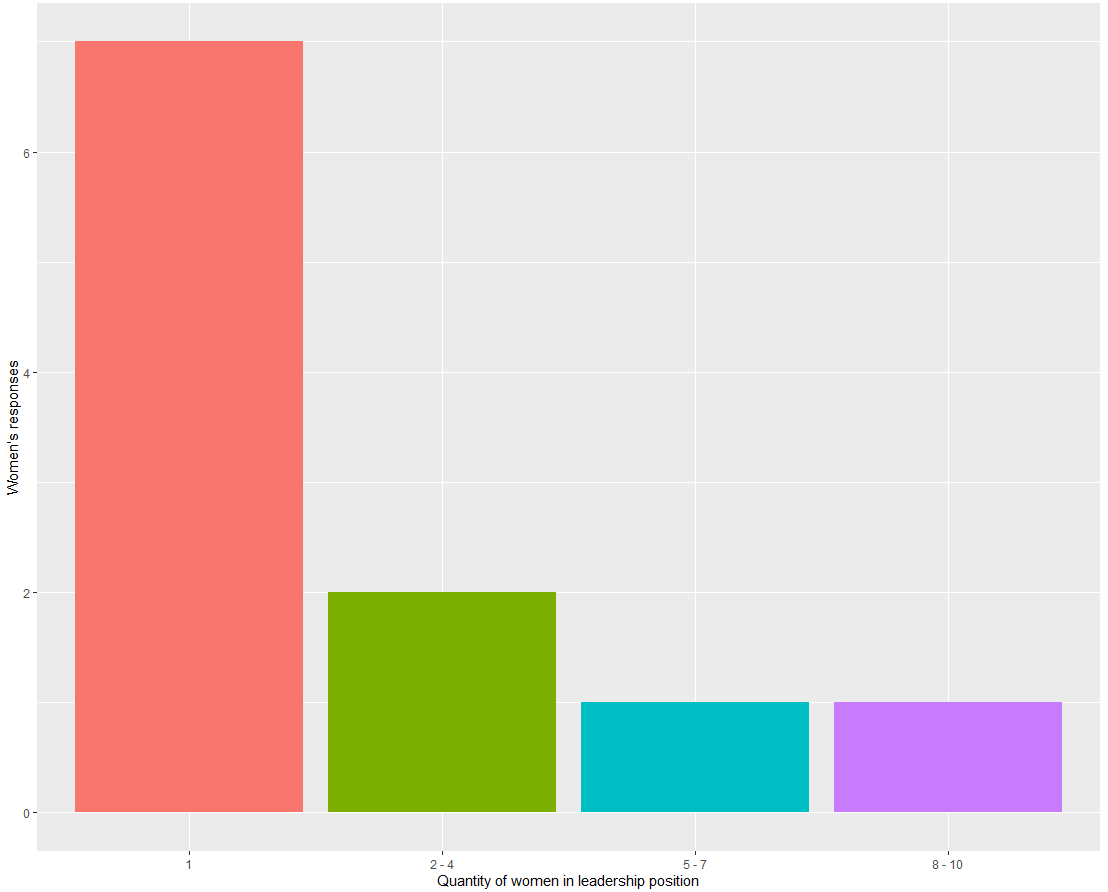
\includegraphics[width=6.0cm]{womenLeadershipPositionColored.png}
    \caption{Women in leadership position}
    \label{fig:leader}
\end{figure}
\end{comment}

%Em relação as características dos projetos que possuem mulheres colaborando (complexidade, duração, número de participantes, linguagem de programação predominante), conforme apresentado na Tabela \ref{tab:profile}, nós podemos concluir que as mulheres entrevistadas colaboram com projetos complexos, com um número de participantes de até 10 pessoas e projetos desenvolvidos nas linguagens JavaScript, Java and Phyton. A maioria das participantes afirmaram que a atividade que elas se sente mais motivadas a realizar em um projeto de desenvolvimento de software, são as atividades de codificação. Esse achado também corrobora com os achados de Izquierdo et al.  \cite{DBLP:journals/software/IzquierdoHSR19}, em que os autores concluíram que a participação das mulheres tem aumentando nas atividades de codificação. 90\%  das entrevistadas mencionaram que estão realizando cursos de capacitação, com o objetivo de aperfeiçoar o seu conhecimento técnico. As entrevistadas acreditam que esses cursos irão facilitar a sua aceitação pelos homens do team, bem como que eles irão respeitar mais o trabalho delas no team.


%Em relação as sugestões das participantes para que a organização tenha um ambiente mais inclusivo para as mulheres, a maioria das mulheres sugeriram promover a diversidade de gênero. A Tabela \ref{tab:inclusive} apresenta as sugestões das 15 entrevistadas. 

\vspace{0.2cm}
\noindent
\textbf{In the literature.} Izquierdo et al. \cite{DBLP:journals/software/IzquierdoHSR19} also identified a low percentage of women in the position of project team leaders at the OpenStack Foundation.

\subsection{Suggestions for inclusiveness}

Regarding the participants' suggestions for the organization to have a more inclusive environment for women, most women suggested promoting gender diversity. Table \ref{tab:inclusive} presents the suggestions of the 15 interviewees. The most recurring topic is to promote gender diversity, that is, fostering activities that could benefit all employees, regardless of their gender. Promoting technical training and coaching activities also seem to be increasingly important to our participants. Although some open source communities have started to adopt such practices (e.g., the Python community was actively seeking a women core developer), these practices do not seem to be well-spread in the software industry that our participants work on. Another suggestion is  to create a code of conduct, so that other team members could refer to and learn how to proper behave. 

%\gnote{tentei descrever um pouco da tabela, mas acho que seria legal descrever um pouco mais, se possivel com alguns quotes.}

\begin{table}[htbp]
    \centering
    \caption{Women's suggestions to improve the organization's environmental to a more inclusive one}
    \label{tab:inclusive}
    \begin{tabular}{p{4.5cm}p{2cm}} 
    \toprule
    \textbf{Suggestions}  & \textbf{Participant}\\ \midrule
    Treat women without any restrictions or privileges & P1 \\
    Promote gender diversity  & P2, P3, P5, P8, P10, P11, P12 and P13   \\ 
    Create a conduct code to decrease the sexist behavioral and jokes & P4 \\
    Promote training and talks about the importance of the equality and diversity of gender & P2 and P6 \\
    Promote technical training, coaching programs, mentoring and sponsorship specific to women & P7, P14 and P15  \\ 
    Define a minimum amount of women in each team  & P9 \\ \bottomrule
    \end{tabular}
\end{table}



\section{Limitations}
\label{limitations}

%Nós encontramos algumas limitações para realizar essa pesquisa. Como as mulheres são subrepresentadas in the fields of Science, Technology, Engineering, and Maths (STEM) \cite{DBLP:conf/icse/Borsotti18,DBLP:journals/ijhcitp/BhattacharyaBM18,DBLP:journals/entropy/BotellaRLM19}, é difícil encontrar mulheres atuando na área de Tecnologia. Dentre as mulheres que encontramos, muitas mulheres não estavam dispostas a participar de entrevistas ou survey em relação aos problemas que elas enfrentam em seu local de trabalho. Nós enviamos e-mail a algumas mulheres e poucas responderam concordando em participar da entrevista. Além disso, as entrevistas ficaram um pouco longas, devido o nosso interesse e necessidade de abordar vários temas. Isso também pode ter desestimulado as participantes. Outra limitação foi que a pesquisa foi focada na percepção das mulheres brasileiras. Assim, nós não podemos generalizar com a percepção das mulheres que atuam em times de desenvolvimento de software de outros países.

There are some limitations related to this research's results, all them related to the sample. Because, women are underrepresented in the fields of Science, Technology, Engineering, and Maths (STEM) \cite{DBLP:journals/entropy/BotellaRLM19}, it is difficult to find women working in the Technology area. Among the women we met, many women were not willing to participate in interviews or surveys due to the problems they face in their workplace. We emailed some women and few replied back willing to participate in the interview.  Another limitation of our sample is the focus on the perception of Brazilian women. Therefore, there are some restrictions about the generalization power of the findings.

%Apesar deste trabalho ter sido desenvolvido com a utilização de uma amostra pequena de participantes, 15 mulheres, o estudo não foi prejudicado, por tratar-se de uma pesquisa qualitativa, e não quantitativa.

\begin{comment}
Although this work was developed with the use of a small sample of participants, 15 women, the study was not harmed, because it is a qualitative rather than a quantitative research.
\gnote{nao entendi bem esse comentario}
\end{comment}

\section{Conclusions}

%Nesse trabalho nós entrevistamos 15 women de diferentes organizações para compreender as suas percepções em relação ao gender bias, desafios e barreiras que elas enfrentam com os membros dos software development teams que elas atuam. Nossos achados revelam que as mulheres são subrepresentadas, atuam em teams com menos de 10 pessoas e que existem poucas mulheres em posições de liderança nos software development teams. Além disso, que é bastante comum elas enfrentarem gender bias por parte dos homens dos teams em que elas atuam. 
What are the barriers and challenges of being a women working on an industry dominated by straight white man?

In this work we interviewed 15 women from different organizations to understand their perceptions regarding gender bias, challenges and barriers that they face with the members of the software development teams that they work with. 

Our findings reveal that women are underrepresented, work in teams of less than 10 people and that there are few women in leadership positions in software development teams. Furthermore, it is quite common for them to face gender bias on the part of the men of the teams in which they work. Women face many barriers, including a lack of trust, credibility, confidence, and recognition. Based on these barriers and challenges, we also propose a set of suggestion to improve inclusiveness in software producing organizations. 

%Como trabalhos futuros, nós pretendemos realizar entrevistas com mulheres de outros Países com o objetivo de verificar se os nossos achados também ocorrem em organizações maiores e com uma cultura diferente. Além disso, também pretendemos entrevistar mulheres que atuam em outras áreas da tecnologia, tais como mulheres que atuam na educação (professoras do ensino superior) e engenharias, para identificar se também ocorre gender bias em outros teams.

\begin{comment}
As future work, we intend to conduct interviews with women from other countries in order to verify whether our findings also occur in larger organizations and with a different culture. In addition, we also intend to interview women working in other areas of technology, such as women working in education (higher education teachers) and engineering, to identify whether gender bias also occurs in other teams.
\end{comment}

\begin{comment}
\section{ACKNOWLEDGMENT}

We are grateful to all women who agreed to participate in this research.
\end{comment}

\bibliographystyle{IEEEtran}
\bibliography{reference}

%It should contain, in the following order, your current position and technical interests, prior applicable professional experience, education, professional affiliations, and address.

\begin{comment}

\begin{IEEEbiography}{Edna Dias Canedo}{\,}is currently an Assistant Professor (tenure track) with the Computer Science Department, UnB. Her current research interests include Software Engineering, Gender issues in software development teams and Software Systems. Canedo received a Ph.D. from University of Bras\'{i}lia, UnB, Brazil. Contact her at ednacanedo@unb.br
\end{IEEEbiography}

\begin{IEEEbiography}{Fabiana Freitas Mendes}{\,}is a Ph.D. candidate at University of Oulu, Finland. She is currently an Assistant Professor in the Faculty of Gama (FGA), UnB. Her current research interests include human aspects in Software Engineering, gender issues in software development teams, and software quality. Contact her at fabianamendes@unb.br
\end{IEEEbiography}

\begin{IEEEbiography}{Anderson Jefferson Cerqueira}{\,}is a Ph.D. student in computing at University of Bras\'{i}lia, UnB, Brazil. He is Professor of Computer Science Course since 2009 and a Military Policeman since 2010. His research interests include Software Engineering, Government Technology and Police Technologies. Contact him at andersonjcdf@gmail.com
\end{IEEEbiography}

\begin{IEEEbiography}{Marcio Vinicius Okimoto}{\,}is currently
pursuing the master's degree in computer science and also a Junior Researcher. His research interests include Mining Software Repositories (MSR) with focus on productivity. Contact him at marciobtos@gmail.com
\end{IEEEbiography}

\begin{IEEEbiography}{Gustavo Pinto}{\,}is an assistant professor of computer science at the Federal University of Par\'{a}, Brazil. His research focuses on the interactions between people and code, spanning the areas of software engineering and programming languages. Pinto received a PhD from Federal University of Pernambuco, Brazil. Contact him at gpinto@ufpa.br
\end{IEEEbiography}
\end{comment}

\end{document}

